%! TeX program = lualatex
\documentclass[a4paper]{article} 

% packages
\usepackage{microtype}      % Slightly tweak font spacing for aesthetics
\usepackage[english]{babel} % Language hyphenation and typographical rules
\usepackage{changepage}     % adjust margins on the fly
\usepackage{booktabs}  % For better-looking tables
\usepackage{pgfplotstable}  % For reading and displaying CSV/TSV files

\usepackage[final, colorlinks = true, urlcolor = black, linkcolor = black, citecolor = black]{hyperref} 
\usepackage{fontspec}
% \setmainfont{EB Garamond}
% \setmonofont[Scale=MatchLowercase]{Deja Vu Sans Mono}

\setmainfont{EB Garamond}[
    Ligatures=TeX,
    Numbers=OldStyle
]

% Fallback font (for missing characters)
\setmainfont{EB Garamond}[
    % Ligatures=TeX,
    % Numbers=OldStyle
]

\newfontfamily{\emojifont}{Noto Color Emoji}[Renderer=Harfbuzz]

% Monospace font configuration
\setmonofont[Scale=MatchLowercase]{DejaVu Sans Mono}

\usepackage[backend=biber, style=numeric, date=iso, urldate=iso]{biblatex}
\addbibresource{references.bib}
\DeclareFieldFormat{urldate}{Accessed on: #1}

\usepackage{minted}
\usemintedstyle{algol_nu}
\usepackage{xcolor}

\usepackage{pgfplots}
\pgfplotsset{width=\textwidth,compat=1.9}

\usepackage{caption}
\newenvironment{code}{\captionsetup{type=listing}}{}
\captionsetup[listing]{skip=0pt}
\setlength{\abovecaptionskip}{5pt}
\setlength{\belowcaptionskip}{5pt}

\usepackage[yyyymmdd]{datetime}
\renewcommand{\dateseparator}{--}

\usepackage{titlesec}
% \titleformat{\section}{\LARGE\bfseries}{}{}{}[\titlerule]
% \titleformat{\subsection}{\Large\bfseries}{}{0em}{}
% \titlespacing{\subsection}{0em}{-0.7em}{0em}
%
% \titleformat{\subsubsection}{\large\bfseries}{}{0em}{$\bullet$ }
% \titlespacing{\subsubsection}{1em}{-0.7em}{0em}

% margins
\addtolength{\hoffset}{-2.25cm}
\addtolength{\textwidth}{4.5cm}
\addtolength{\voffset}{-3.25cm}
\addtolength{\textheight}{5cm}
\setlength{\parskip}{0pt}
\setlength{\parindent}{0in}
% \setcounter{secnumdepth}{0}

\begin{document}
\hrule \medskip
\begin{minipage}{0.295\textwidth} 
    \raggedright
    \footnotesize 
    \begin{tabular}{@{}l l}
        Name: & Andrew Hayes \\
        Student ID: & 21321503 \\
        E-mail: & \href{mailto://a.hayes18@universityofgalway.ie}{\texttt{a.hayes18@universityofgalway.ie}} \\
    \end{tabular}
\end{minipage}
\begin{minipage}{0.4\textwidth} 
    \centering 
    \vspace{0.4em}
    \LARGE
    \textsc{ct437} \\ 
\end{minipage}
\begin{minipage}{0.295\textwidth} 
    \raggedleft
    \today
\end{minipage}
\medskip\hrule 
\begin{center}
    \normalsize
    Assignment 2: Using \& Benchmarking Block Ciphers with OpenSSL
\end{center}
\hrule
\medskip

\section{Block Cipher Benchmarking}
\begin{table}[H]
    \centering
    \pgfplotstabletypeset[
        col sep=tab, % Specifies that the file is tab-separated
        string type, % Ensures text columns are treated correctly
        header=true, % Includes the header row
        columns/Cipher/.style={column name=Cipher},
        columns/Key Size/.style={column name=Key Size (bits)},
        columns/Mode/.style={column name=Mode},
        columns/Data Size (MB)/.style={column name=Data Size (MB)},
        columns/Encryption Time (s)/.style={column name=Encryption Time (s)},
        columns/Decryption Time (s)/.style={column name=Decryption Time (s)},
        every head row/.style={before row=\toprule, after row=\midrule},
        every last row/.style={after row=\bottomrule}
    ] {../code/results.tsv} % Filename
    \caption{Benchmarking results from TSV file}
\end{table}

To benchmark the CPU time of my program, I used the standard POSIX \mintinline{c}{getrusage()} function declared in the \mintinline{c}{<sys/resource.h>} header, and wrote the collected experimental data to a tab-separated value (TSV) file defined in my \verb|benchmark.h| header file, as I generally prefer TSV to CSV due to its increased human-readability in plaintext form.
I made sure to only open and write to the results file \textit{after} each benchmark had been measured to ensure that the data was accurate.
The above table of results is generated automatically from the TSV file using the {\LaTeX} \mintinline{latex}{pgfplots} package, and the below bar charts were generated using a simple Python script.
Since I already run a Linux-based operating system on my laptop, I was able to run these benchmarks natively on my machine, both making it slightly easier for me to run the tests but also likely greatly improving the performance of the block ciphers as the program had full access to my system resources instead of limited virtualised hardware.

\begin{figure}[H]
    \centering
    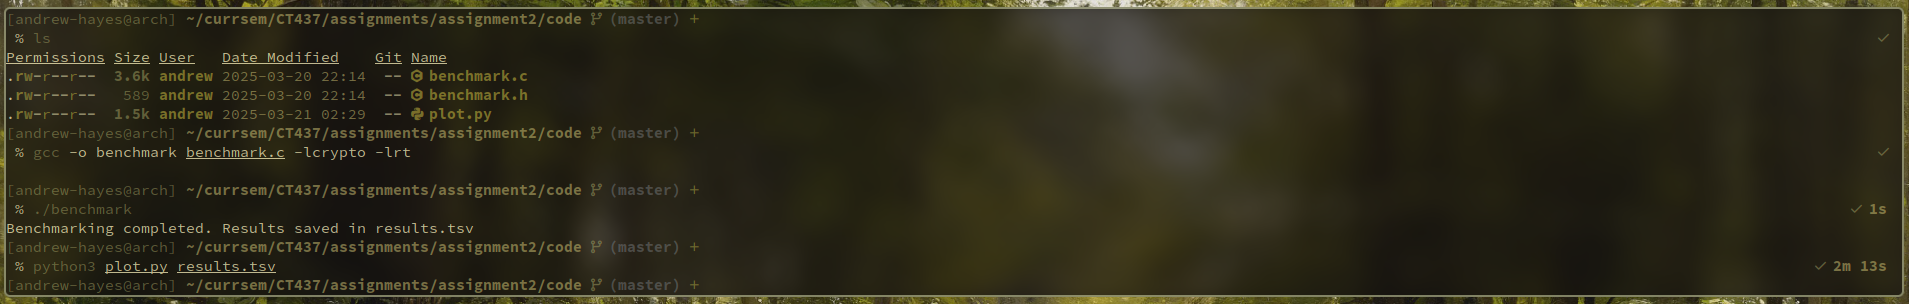
\includegraphics[width=\textwidth]{./images/one.png}
    \caption{ Compiling and running the benchmarking program }
\end{figure}

\begin{figure}[H]
    \centering
    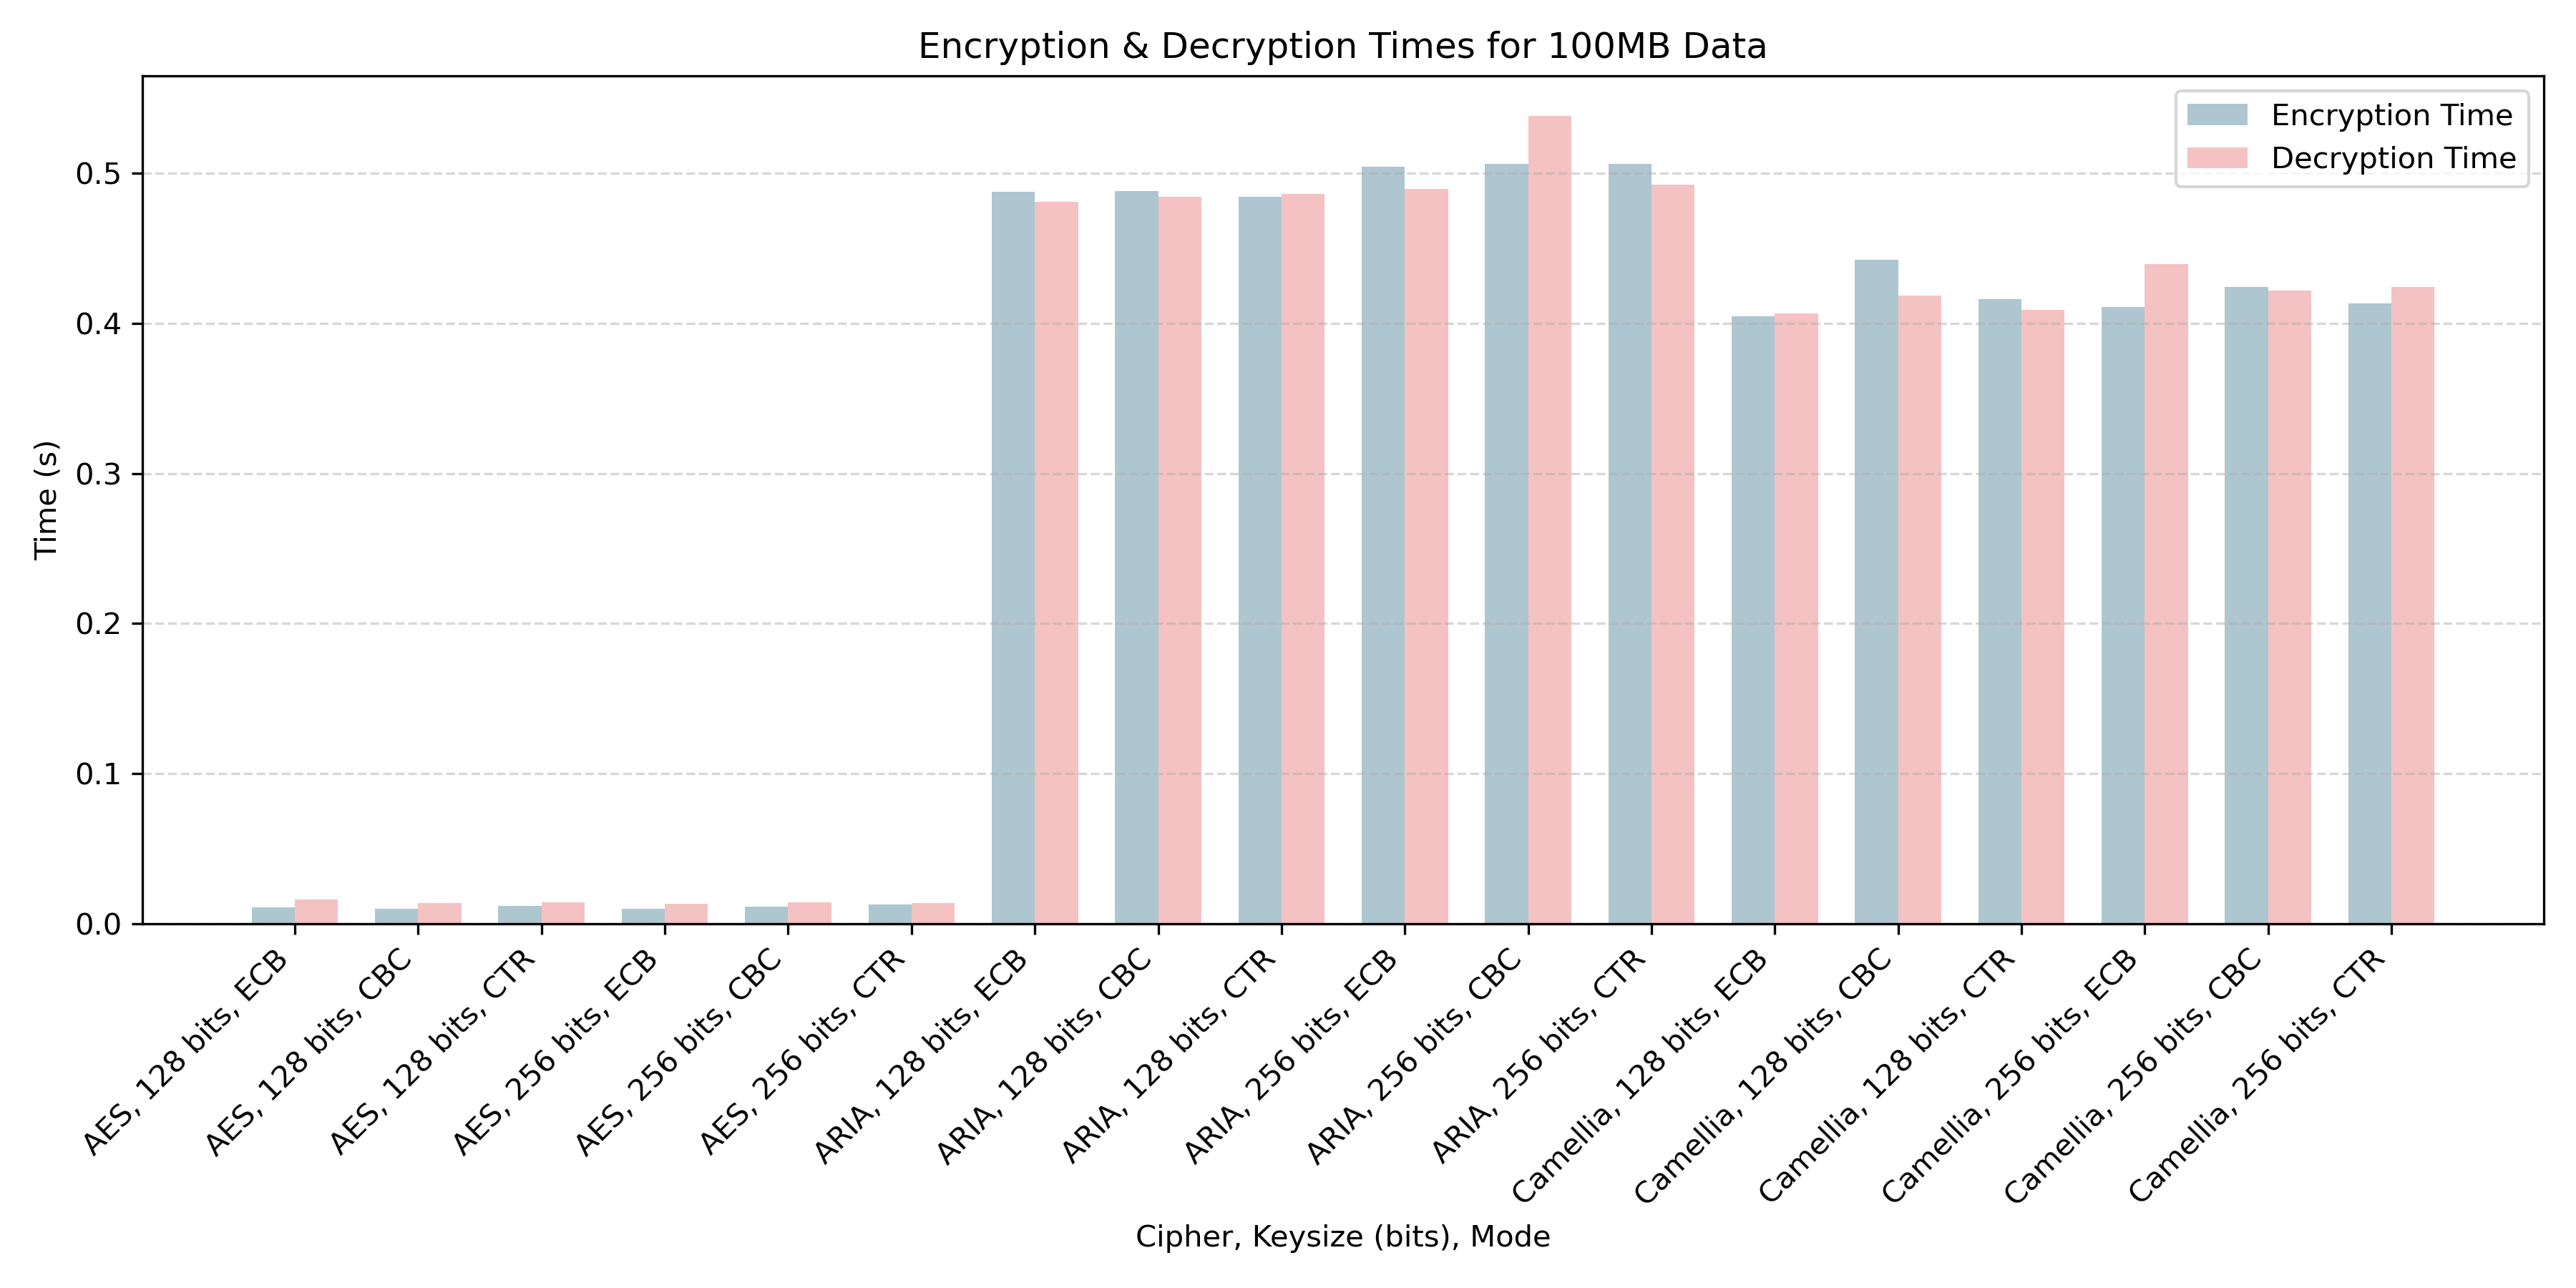
\includegraphics[width=\textwidth]{./images/100mb.png}
    \caption{Encryption \& decryption times for 100MB data}
\end{figure}

\begin{figure}[H]
    \centering
    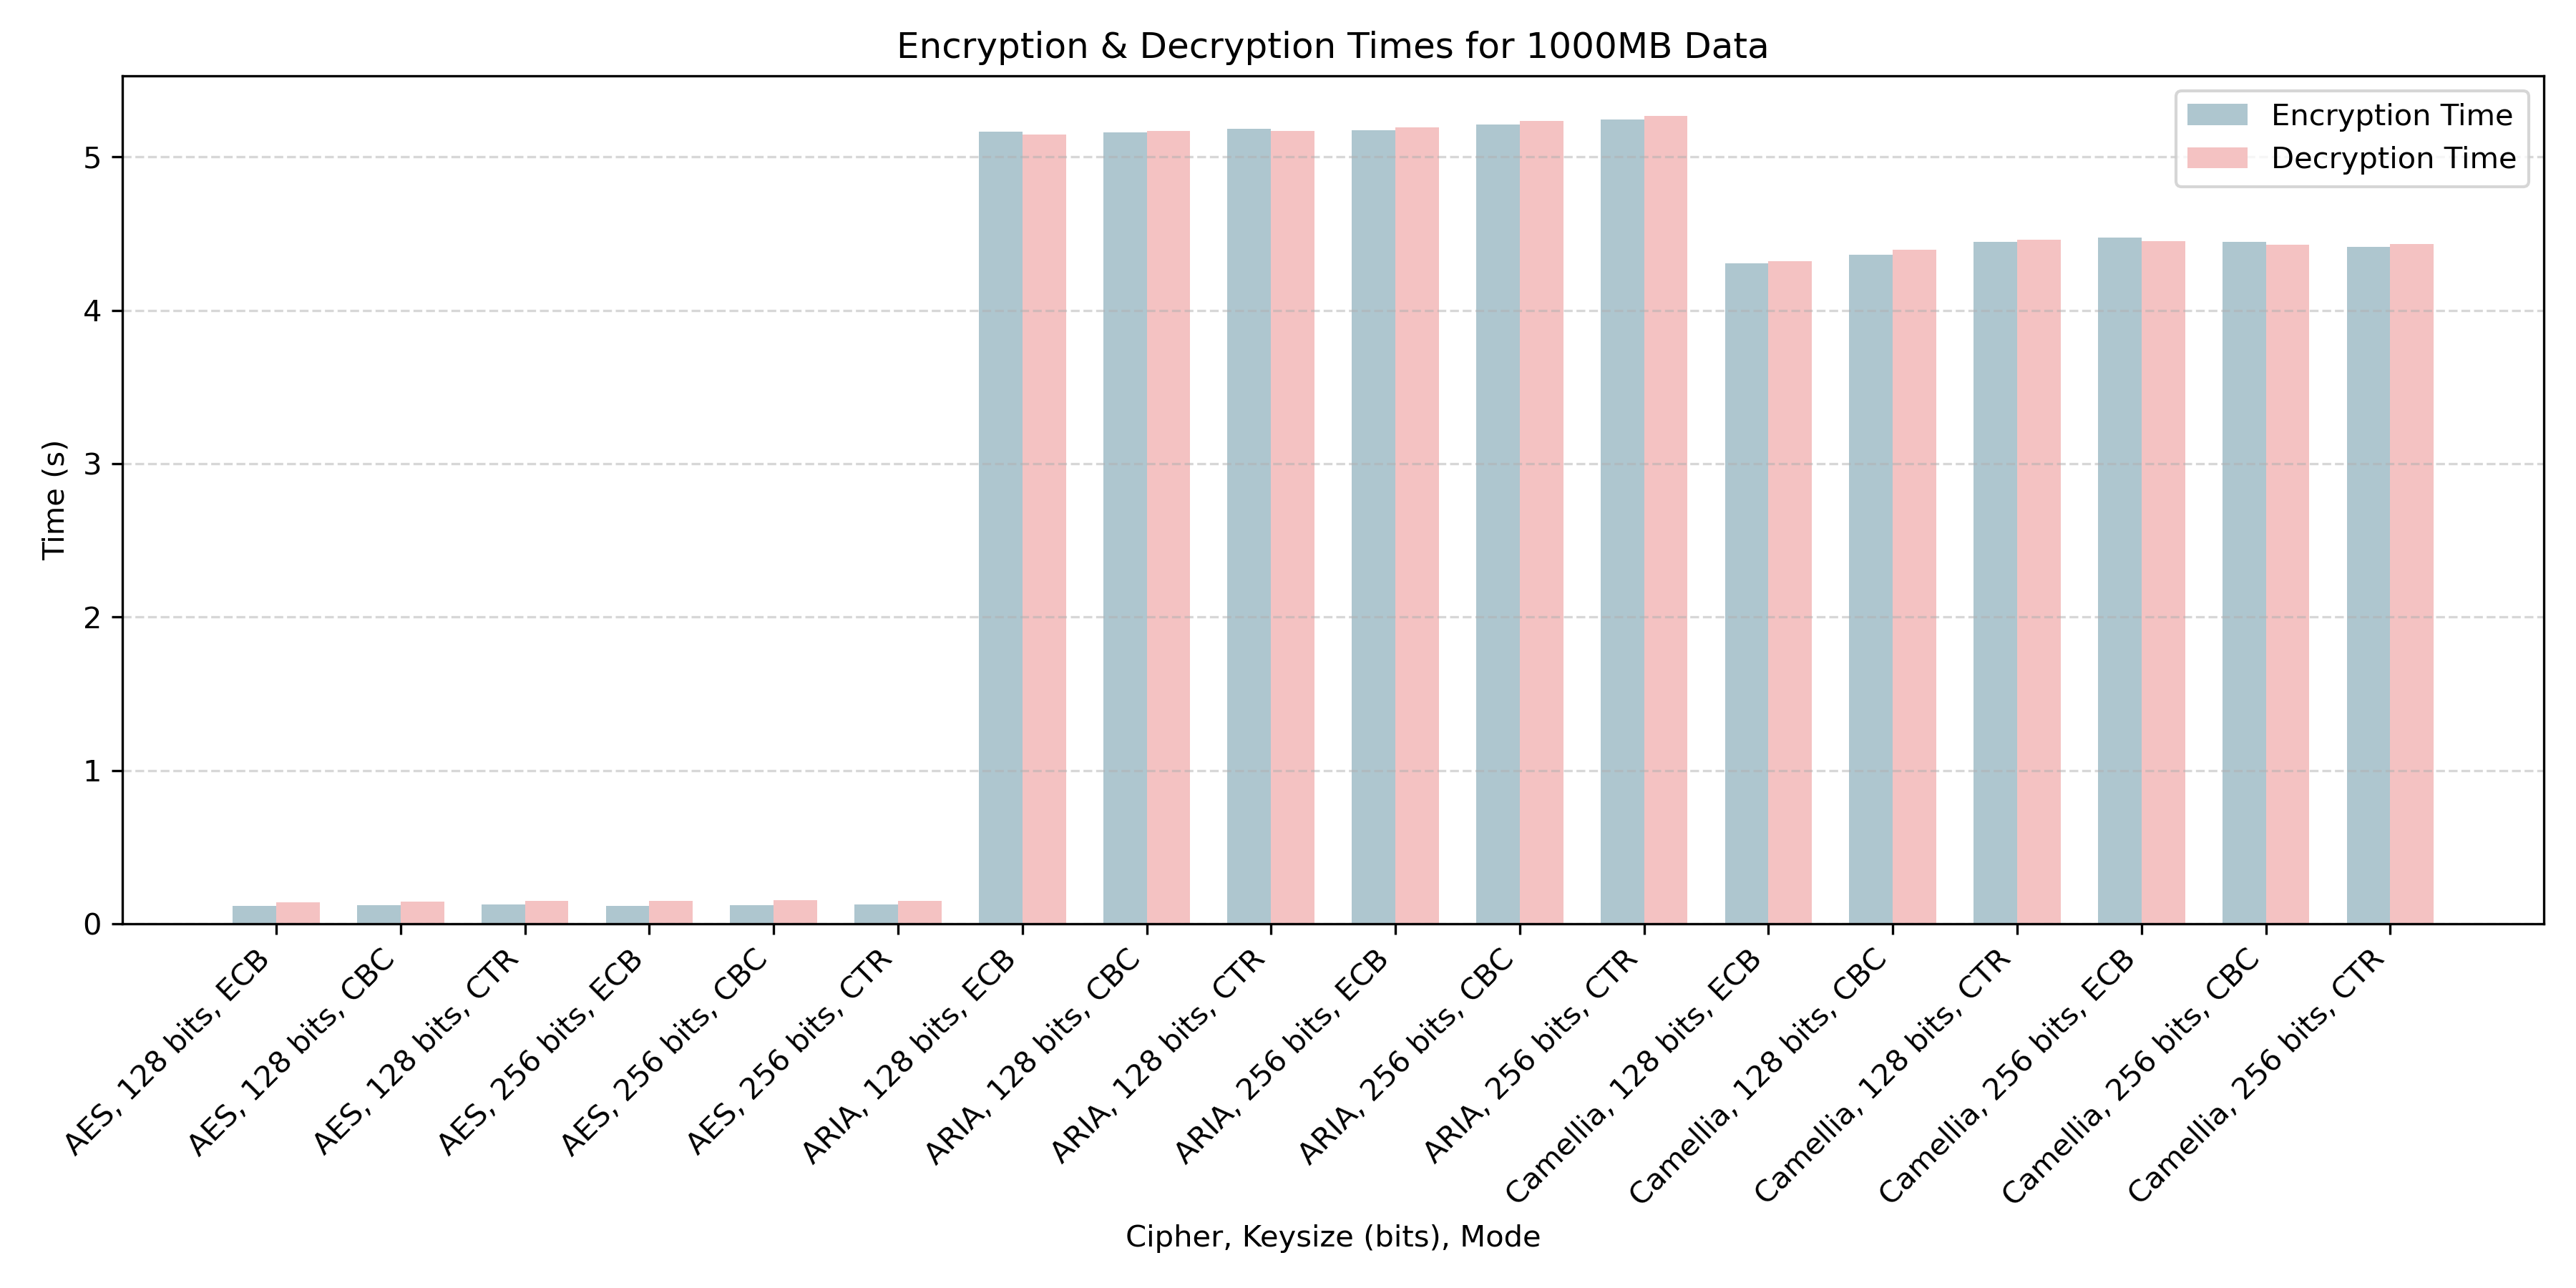
\includegraphics[width=\textwidth]{./images/1000mb.png}
    \caption{Encryption \& decryption times for 1000MB data}
\end{figure}

The above bar charts contain the time taken for encryption \& decryption for each cipher, key size, \& mode combination tested;
the blue columns represent the time taken for encryption and the red columns represent the time taken for decryption.
The graphs are separated by the size of the data being encrypted / decrypted.
What is most immediately obvious to me when looking at these two graphs is how similar the two are:
the results and relative scaling look almost identical until you look at the $y$-axis and see that each time result is about 10 times higher in the 1000MB experiment than in the 100MB experiment, which makes perfect sense, as the one experiment involves 10 times the data of the other.
Since block ciphers process only fixed-size blocks, processing each block (theoretically) takes a constant amount of time, and so the CPU time of the algorithm will scale linearly with the amount of data to be encrypted or decrypted.
\\\\
The next feature of the bar charts that is immediately obvious is that the blue columns are approximately the same height as the red columns: encryption time $\approx$ decryption time.
This is what one would expect, as the block ciphers in question are \textbf{symmetric}: the operations used for encryption \& decryption are inverses of each other.
The slight variations in some results can be attributed to fluctuations in background processes consuming CPU on my laptop when I ran the tests.
The one exception here are the AES results:
relative to the amount of time taken by encryption for the AES results, the decryption results are quite a bit higher.
Furthermore, the decryption results are consistently higher than the encryption results, unlike the other algorithms where it appears to be more or less random noise.
This is because of \textbf{AES-NI} (Advanced Encryption Standard New Instructions): a set of hardware instructions on Intel/AMD CPUs that allow hardware acceleration of AES operations.
OpenSSL automatically detects if AES-NI is supported at runtime, and will automatically take advantage of these hardware accelerations if available.
On Linux-based operating systems, you can check if your CPU has AES flags in its CPU information to check if AES-NI is supported by running \mintinline{shell}{grep -c aes /proc/cpuinfo}.

\begin{figure}[H]
    \centering
    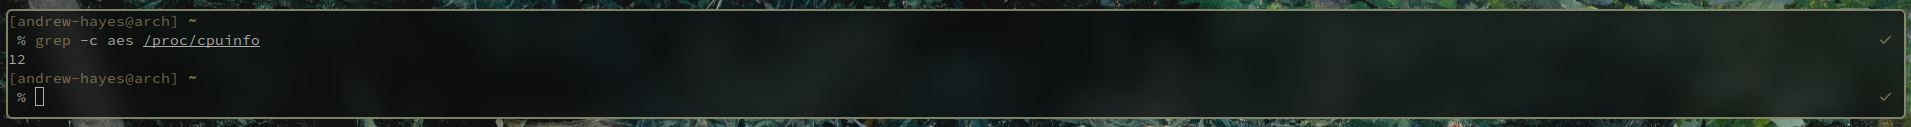
\includegraphics[width=\textwidth]{./images/aesni.png}
    \caption{Output of \mintinline{shell}{grep -c aes /proc/cpuinfo} showing that my CPU supports AES-NI}
\end{figure}

As can be seen from the terminal screenshot above, my laptop's CPU does indeed support AES-NI, which explains not only the slightly slower (relatively speaking) AES decryption times, but also why the AES times are so much faster than both the ARIA and Camellia times.
Ordinarily, for similar amounts of data, one would expect that AES would take roughly the same amount of time as ARIA or Camellia, and possibly be outperformed by something like Camellia as AES has more lookup tables \& transformations than Camellia, which can be costly in software implementations.
However, since my CPU has hardware-acceleration for AES operations with AES-NI, these operations occur in the hardware rather than the software, and are therefore much, much faster.
\\\\
We can also see from the bar charts that ARIA is consistently slower than Camellia;
as there is no hardware acceleration for either, this is down purely to their software implementations / algorithmic design.
This can be explained by the fact that ARIA has a computationally intensive round function that uses a substitution-permutation network structure (like AES) with multiple layers of S-box substitutions, diffusion matrices, \& key-dependent transformations.
On the other hand, Camellia uses a Feistel network which is more lightweight and better-suited for software execution.
\\\\
If you look carefully at the graphs, you can see that encryption \& decryption with a 256-bit key is just slightly slower than encryption \& decryption with a 128-bit key.
A larger key size means more encryption rounds and more computation per block, thus making using 256-bit key slower than a 128-bit key.
However, this speed decrease is usually well worth it, as it makes the encryption far stronger and much more difficult to brute force.
\\\\
The last aspect of the bar charts to discuss is the impact of the various modes on encryption \& decryption time.
The differences here are the most difficult to see in the bar charts but are there if you look closely; they may be easier to see in the tabulated results.
\begin{enumerate}
    \item   ECB mode is the fastest of the three modes because each block is encrypted independently with no chaining or initialisation vector required, making it simple \& fast, and easy to parallelise in both encryption \& decryption.
            However, it is not particularly secure: identical plaintext blocks will result in identical ciphertext blocks, and it can leak data patterns in the encrypted data.

    \item   CTR mode is the second fastest, as it works by converting the block cipher into a stream cipher and uses a counter \& a nonce to generate a keystream.
            It encrypts the counter, then \verb|XOR|s it with the plaintext.
            This is highly parallelisable for both encryption \& decryption, and uses the same logic for both.
            It is also much more secure than ECB mode, as the counter never repeats.

    \item   The slowest of the three modes is CBC mode:
            in CBC mode, each plaintext block is \verb|XOR|ed with the previous ciphertext block before encryption, requiring an IV for the first block.
            This makes it more secure than ECB as it removes repeating patterns, but it is not parallelisable as each block depends on the previous, making encryption much slower.
            However, decryption can be parallelised somewhat, as ciphertext blocks can be decrypted independently before they are \verb|XOR|ed with the previous ciphertext block, but it is not clear from the results whether or not such parallelisation was utilised, and if it was, it had little impact on the performance.
\end{enumerate}

\section{Implementing \& Benchmarking Triple-DES}
\begin{table}[H]
    \centering
    \pgfplotstabletypeset[
        col sep=tab, % Specifies that the file is tab-separated
        string type, % Ensures text columns are treated correctly
        header=true, % Includes the header row
        columns/Cipher/.style={column name=Cipher},
        columns/Key Size/.style={column name=Key Size (bits)},
        columns/Mode/.style={column name=Mode},
        columns/Data Size (MB)/.style={column name=Data Size (MB)},
        columns/Encryption Time (s)/.style={column name=Encryption Time (s)},
        columns/Decryption Time (s)/.style={column name=Decryption Time (s)},
        every head row/.style={before row=\toprule, after row=\midrule},
        every last row/.style={after row=\bottomrule}
    ] {../code/3des_results.tsv} % Filename
    \caption{Benchmarking results from TSV file}
\end{table}

\begin{figure}[H]
    \centering
    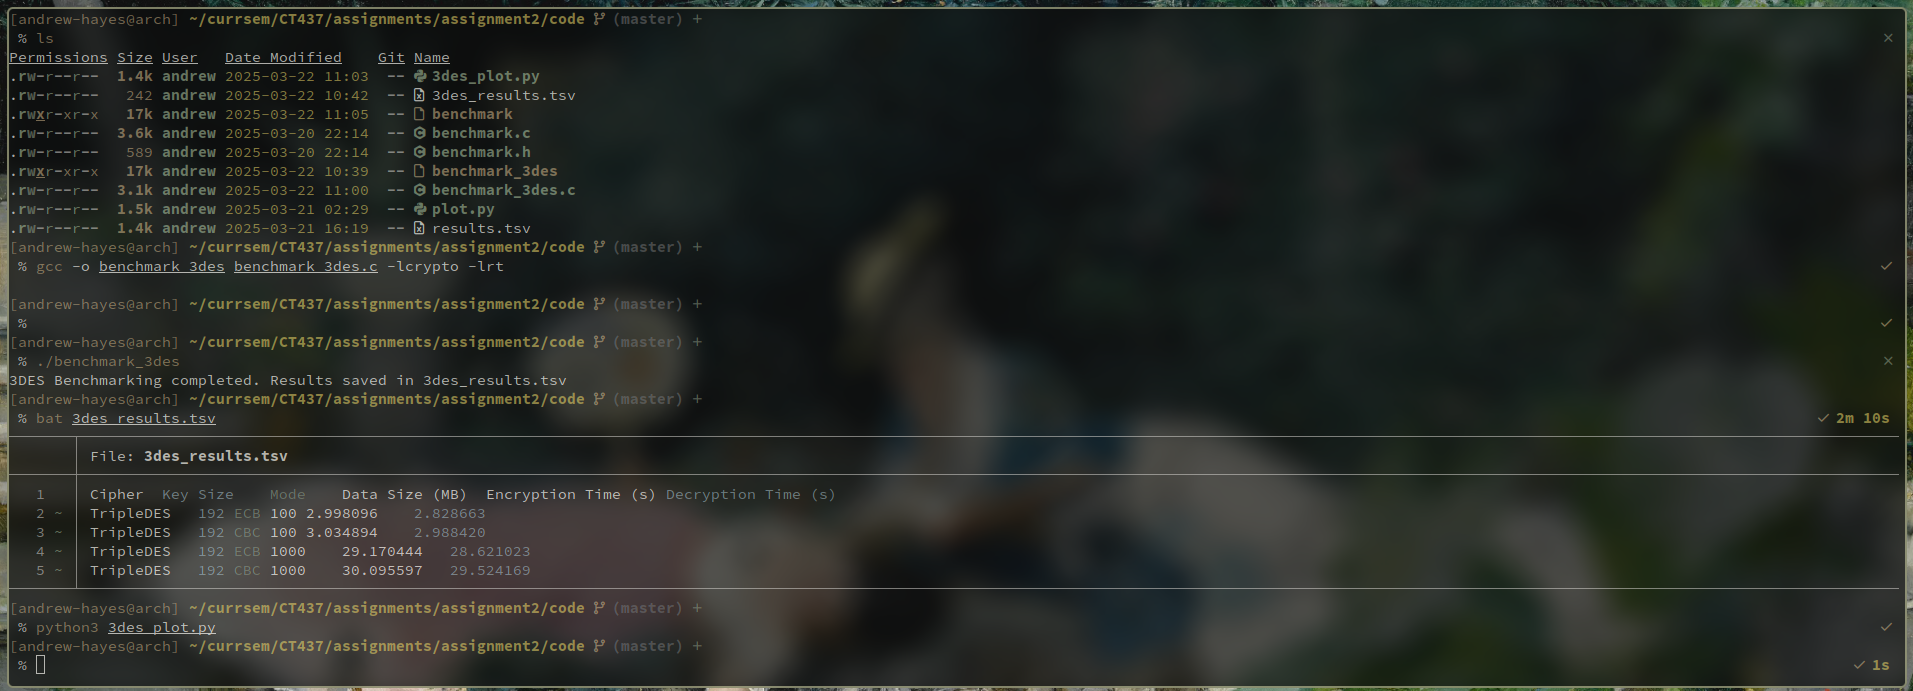
\includegraphics[width=\textwidth]{./images/3desss.png}
    \caption{Compiling \& running the benchmarking program}
\end{figure}

\begin{figure}[H]
    \centering
    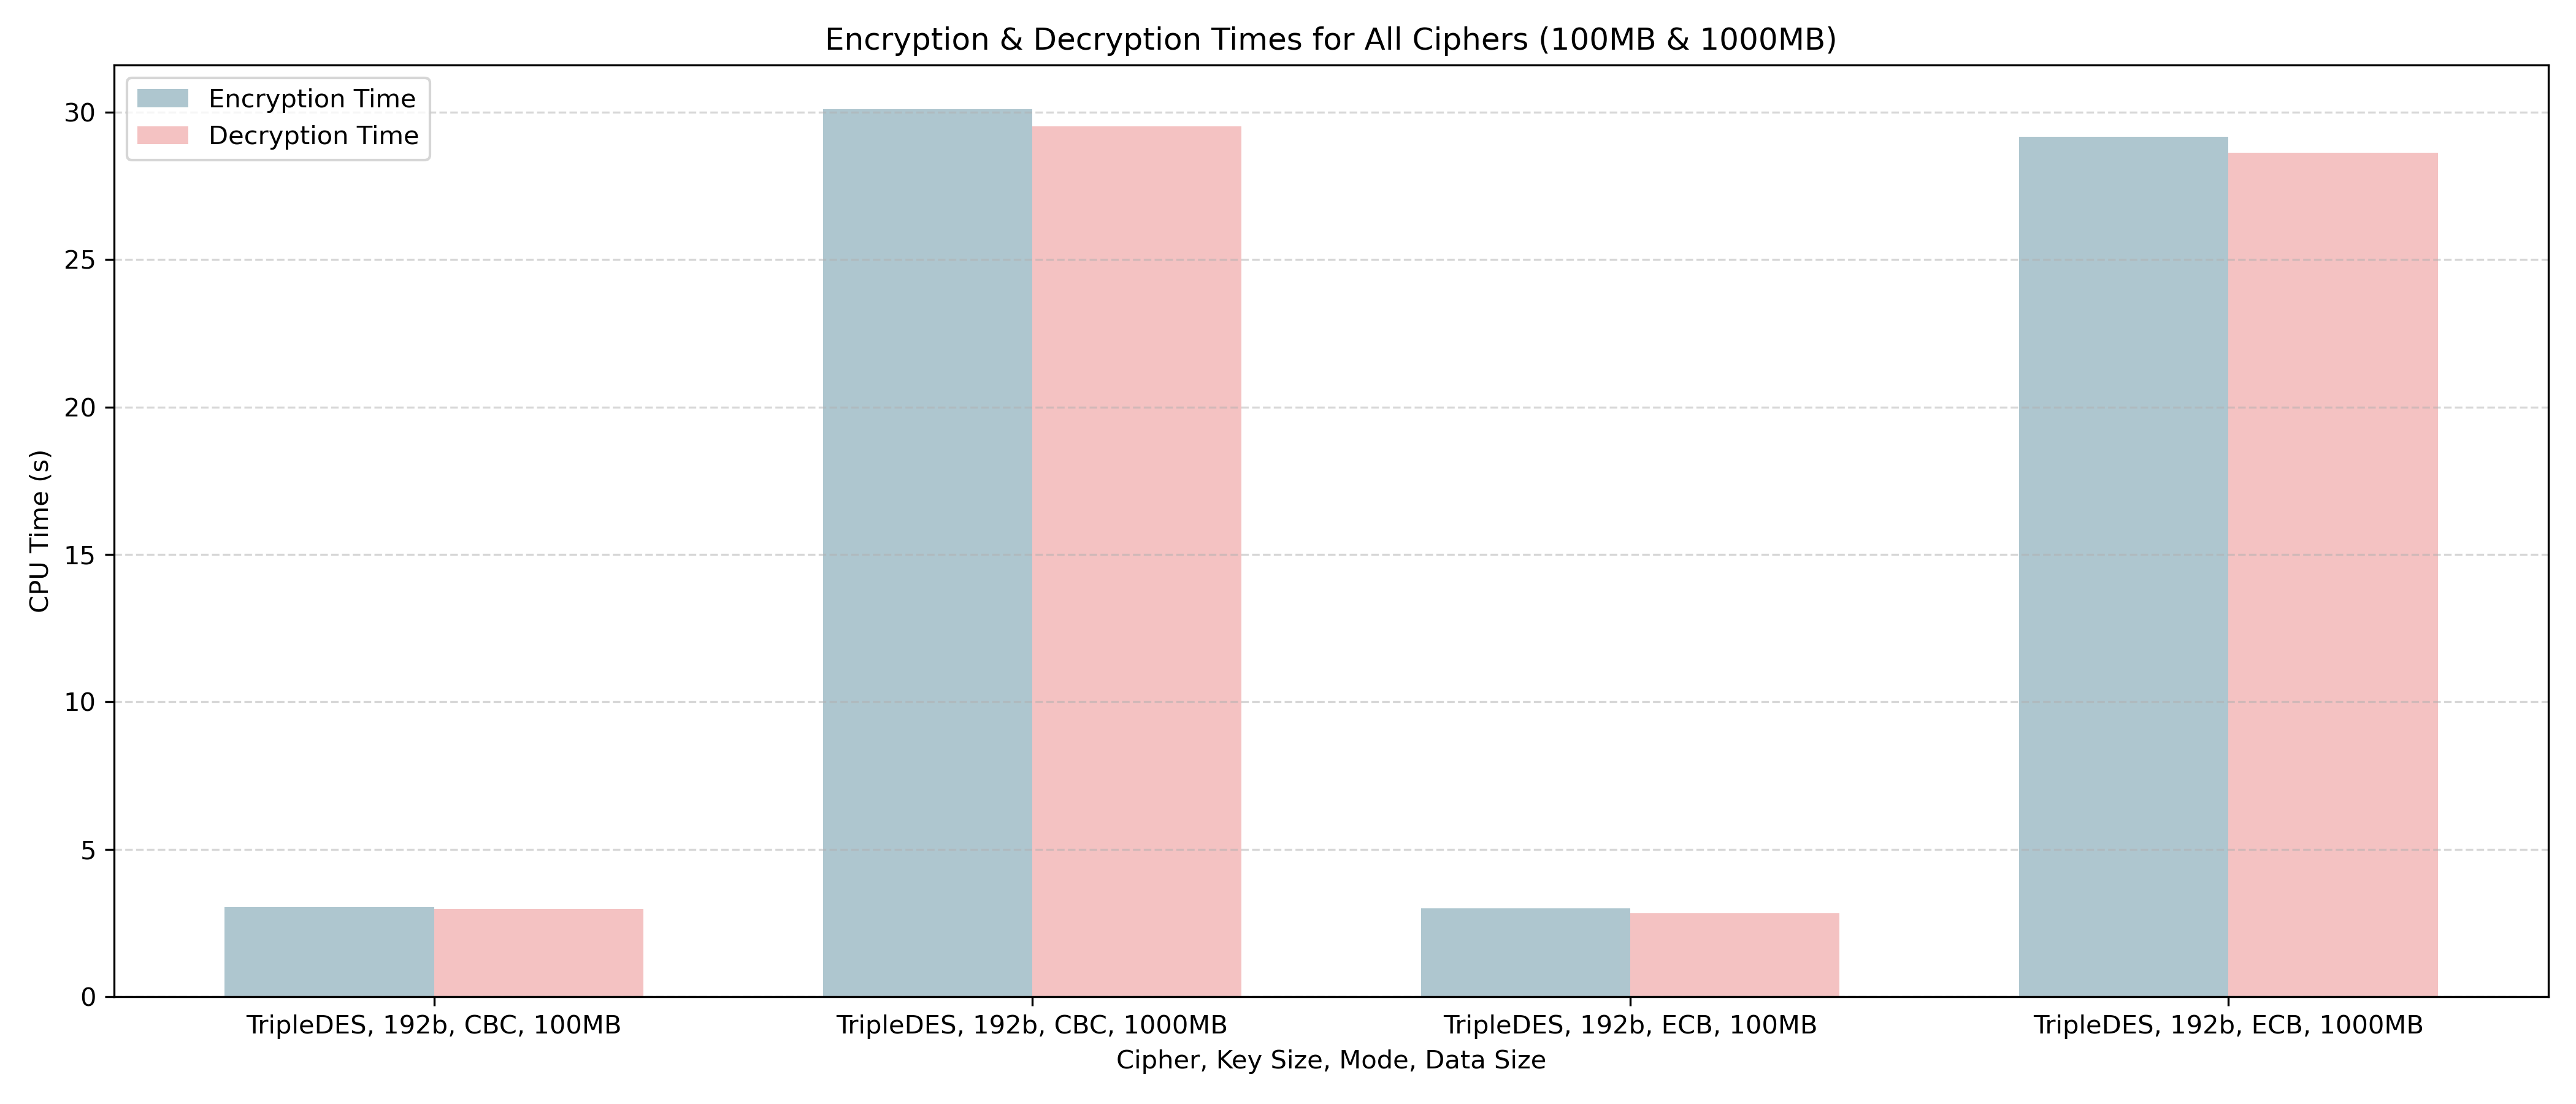
\includegraphics[width=\textwidth]{./images/3des.png}
    \caption{Encryption \& decryption times for Triple-DES}
\end{figure}

As before, what is immediate obvious about this graph is that the times for 1000MB of data are pretty much exactly 10 times that of the times for 100MB of data, as Triple-DES is a block cipher and so the computational time scales linearly with input data size.
We can also see that decryption is generally a little faster than encryption but is more or less the same speed. 
This is likely due in part due to background noise, but is also possibly due to internal caching behaviour or other optimisations for decryption in the OpenSSL implementation.
In general, however, one would expect encryption \& decryption to take more or less the same amount of time, as Triple-DES is a symmetric algorithm and therefore decryption requires the same steps as encryption, just inverted.
As before, since ECB encrypts each block independently, it is faster than CBC due to being parallelisable, whereas CBC has dependency between blocks and is therefore not parallelisable and thus slower.
\\\\
The main comparison to be drawn from comparing the Triple-DES results to the results from the first experiment is that Triple-DES is much slower, taking 5--10 times more time to execute than any other algorithm from the first experiment.
This is down to three primary reasons: DES operates on 64-bit blocks which is less efficient, is very outdated so has no hardware acceleration and not much software optimisation, and because Triple-DES runs DES three times, so it's automatically going to be 3 times slower.
For example Triple-DES took about 6 times longer to run than Camellia in ECB mode on 1000MB of data: $\sim$30 seconds versus $\sim$5 seconds.
This makes sense, as we would expect DES to be about twice as slow as Camellia and, Triple-DES will naturally be three times slower than DES, adding up to a 6$\times$ speed decrease.



\end{document}
